\section{Entwurfsmuster (8P)}
\task{2 unterschiedliche Entwurfsmuster aus der Vorlesung (oder nach Absprache auch andere) jeweils benennen, sinnvoll einsetzen, begründen und UML-Diagramm}
\subsection{Entwurfsmuster : Singleton (Erzeugungsmuster) (4P)}
\textbf{Einsatz im Projekt:} \texttt{Localization}-Klasse (\texttt{org.bilanzius.utils.Localization})

\lstinputlisting[
    language=Java,style=codeStyle]{kapitel8_entwurfsmuster/code/Singleton.java}

\subsection*{Sinnvoller Einsatz}
Die \texttt{Localization}-Klasse wird einmalig instanziiert und stellt eine globale Instanz bereit, die für das Abrufen von sprachabhängigen Texten zuständig ist. So kann das gesamte System konsistent auf Sprachdaten zugreifen, ohne dass mehrere Objekte unterschiedliche Zustände haben.

\subsection*{Begründung}
\begin{enumerate}
    \item Nur eine Instanz notwendig für zentrale Konfiguration
    \item Globale Zugänglichkeit
    \item Minimierung von Speicherverbrauch und Inkonsistenzen
\end{enumerate}

\subsection*{UML-Diagramm}
\begin{figure}[htbp]
    \centering
    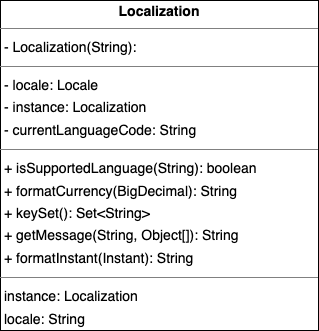
\includegraphics[width=0.5\linewidth]
    {kapitel8_entwurfsmuster/UMLs/localizaition.drawio.png}
\end{figure}

\subsection{Entwurfsmuster: Strategy (Verhaltensmuster) (4P)}

\textbf{Einsatz im Projekt:} Datenbankdienste wie \texttt{BankAccountService} \& \texttt{SqliteBankAccountService}

\subsection*{Sinnvoller Einsatz}
Im \texttt{DatabaseProvider} wird zur Laufzeit entschieden, welche konkrete Datenbankimplementierung (\texttt{SqliteBankAccountService}, \texttt{SqliteCategoryService} usw.) verwendet wird. Dies erfolgt über das Interface \texttt{BankAccountService}, \texttt{CategoryService}, etc.

\subsubsection*{DatabaseProvider:}
\lstinputlisting[
    language=Java,style=codeStyle]{kapitel8_entwurfsmuster/code/dbprovider.java}

\subsubsection*{BankAccountService:}
\lstinputlisting[
    language=Java,style=codeStyle]{kapitel8_entwurfsmuster/code/accountService.java}


\subsection*{Begründung}
\begin{enumerate}
    \item Flexible Austauschbarkeit von Algorithmen (hier: DB-Strategien)
    \item Gute Erweiterbarkeit
    \item Unterstützung von losen Kopplungen und Testbarkeit
\end{enumerate}

\subsection*{UML-Diagramm}
\begin{figure}[htbp]
    \centering
    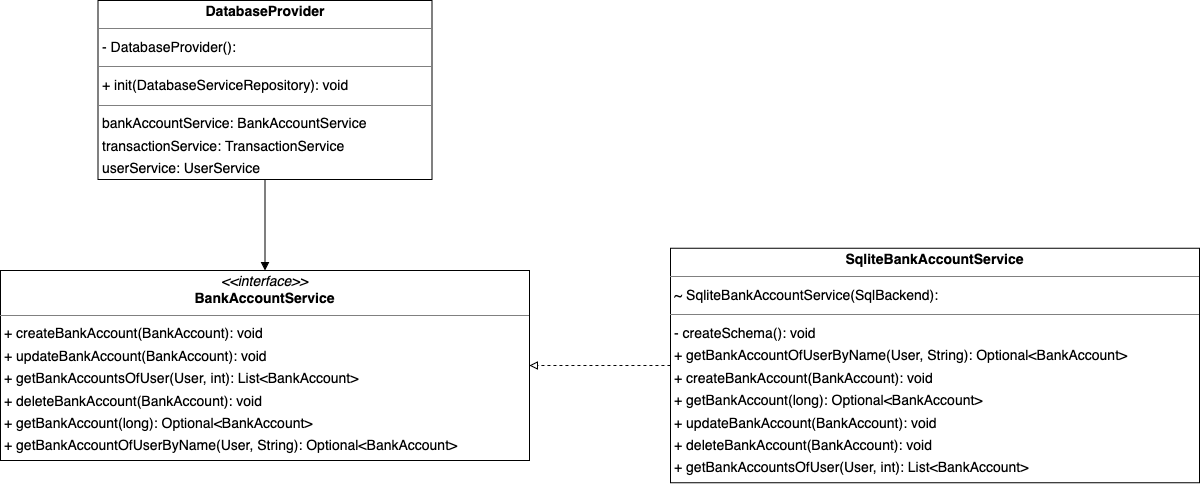
\includegraphics[width=\linewidth]
    {kapitel8_entwurfsmuster/UMLs/db.drawio1.png}
\end{figure}